The system to be developed is inserted in a network, more specifically, an infrastructure based network, as shown in figure \ref{fig:infr_based_arch}. This type of networks are composed by wireless segments of a more extensive network, whose core is usually a wired network. Infrastructure-based networks have a special station, called an \ac{ap} or \ac{bs}, which serves as an interface between the wireless segment and the rest of the network. Inside the wireless segment, there will be a centralized communication, so that all messages that circulate on the network pass through a central station. That way, the network only supports two transmission directions: the downward direction (downlink), from the base station to the other stations, and the uplink direction, from the stations to the base station. The downlink usually allows the simultaneous transmission of information to a group of stations in the cell (multicast) or to all stations (broadcast).

\begin{figure}[ht]
	\centering
	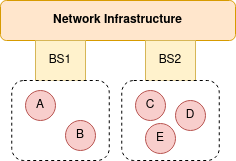
\includegraphics[width=.36\textwidth]{/03system_overview/infrastructure_based}
	\caption{Infrastructure based network architecture.}
	\label{fig:infr_based_arch}
\end{figure}

Street lighting is generally divided into sectors, facilitating maintenance and problem solving regarding the lighting network. In figure \ref{fig:network_arch}, one can see that the base station is a “special station”, since it connects the local network of lighting poles to other base stations, through a remote server, and also because it has a camera for the detection of available parking spaces. The rest of the stations that compose the local network, the local systems, will only do the smart management of their lamps.

\begin{figure}[ht]
	\centering
	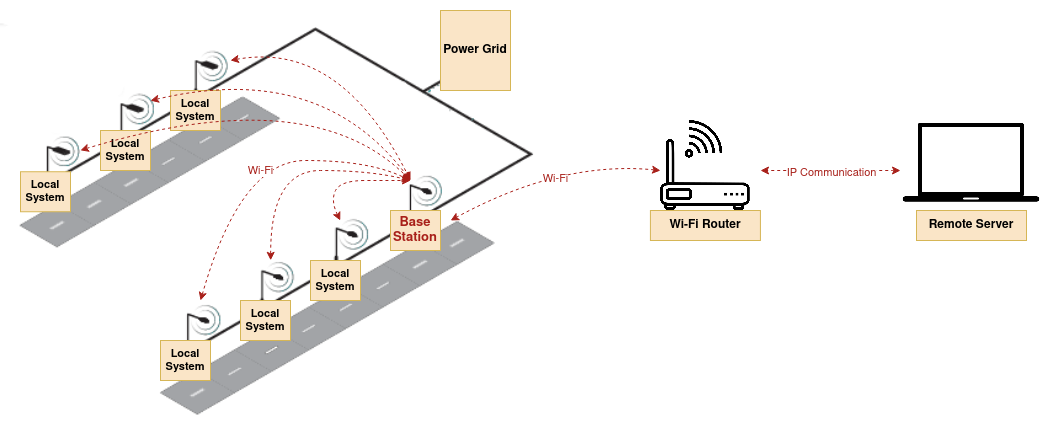
\includegraphics[width=1\textwidth]{/03system_overview/network_arch}
	\caption{Network architecture.}
	\label{fig:network_arch}
\end{figure}

The range of a Wi-Fi network depends primarily on the number and type of wireless access points used to build it, and so, the cost to build and maintain these networks increases significantly as the range increases.

The Wi-Fi signal range of any given access point also varies significantly from device to devices, depending on the specific 802.11 protocol that its used, the strength of its device transmitter and the nature of physical obstructions or radio interferences in the surrounding area. Also, due to laws of physics, 5 GHz Wi-Fi connections are more susceptible to obstructions than are 2.4 GHz. Generally, Wi-Fi routers operating on the traditional 2.4 GHz band reach up to 46 meters indoors and 92 meters outdoors. \cite{wi_fi_range}

Using a router running 802.11n, in open space the wi-fi signal range can be a little over 60 meters. \cite{wi_fi_802_11n} That being said, if each lamppost is spaced by 4 meters, each base station can easily connect with 10 local systems. To communicate with a remote server, the router will be connected to the internet through an Ethernet cable, or similar, that will most certainly already exist near the lampposts, in the telecommunications infrastructure.

